\documentclass[a4paper]{article}
\usepackage[utf8]{inputenc}
\usepackage[T1]{fontenc}
\usepackage{graphicx}
\usepackage[slovene]{babel}
\begin{document}
\title{Definicijsko območje in zaloga vrednosti}
\maketitle
\[f(x)=\log(|\sqrt{1-x^2}-2|-\frac{3}{2})\]
\begin{itemize}

\item najprej izračunajmo definicijsko območje znotraj logaritma.
\(\sqrt{1-x^2}\) bo definiran ko bo $1-x^2>0\rightarrow 1>x^2\leftrightarrow |x|<1$
\\
\item sedaj se osredotočimo na absolutno vrednost $|\sqrt{1-x^2}-2|$ in upoštevajmo da vemo da je $|x|<1$

hitro se vidi da je $|\sqrt{1-x^2} |$ vedno manjši kvečjemu enak 1 ko je $|x|<1$ (lahko narišeš graf ali pa rešiš enačbo$\sqrt{1-x^2}-2=0$ in vidiš da je $\sqrt{1-x^2}-2$ vedno manjše od 0 ko je  $|x|<1$)\\
zato bo $|\sqrt{1-x^2}-2|=2-\sqrt{1-x^2}$
\\

naša enačba ima sedaj obliko\[f(x)=\log(2-\sqrt{1-x^2}-\frac{3}{2})=\log(\frac{1}{2}-\sqrt{1-x^2})\]

\item sedaj zračunamo kdaj bo $\frac{1}{2}-\sqrt{1-x^2}>0$ sa je logaritem definiran takrt ko je tisto znotraj njega več kot 0

koren damo na eno stran. Potem kvadriramo in dobimo rešitve $x\in(-1,\frac{\sqrt{3}}{2})\lor(\frac{\sqrt{3}}{2},1)$ in to je potem našo definicijsko območje

\item zalogo vrednosti: vemo da je logaritemska funkcija naraščajoča zato bo svoj maks dosegla takrat ko bo tisto znotraj največje.To je pri nama ko bo x=1 ali x=-1 in takrat bo $f(1)=\log(\frac{1}{2})$ \\
 minimum pa takrat ko bo tisto znotrja najmanjše kar je pri nama ko je $x=\frac{\sqrt{3}}{2}\lor x=-\frac{\sqrt{3}}{2}\rightarrow f(\frac{\sqrt{3}}{2})=\log(1/2-\sqrt{1-(\frac{\sqrt{3}}{2})^{2}} =)\log(0)=-\infty$ Tuki bi mogoč lahko kdo komplciral ker $\frac{\sqrt{3}}{2}$ ni v definicijskem območju vendar ko se vrednosti približujejo $\frac{\sqrt{3}}{2}$ je logaritem poljubno blizu 0
 
 iz tega sledi da je zaloga vrednosti te funkcije od $(-\infty,\log(\frac{1}{2})$
 \textbf{opomba: } Zalogo vrednosti lahko ponavadi zračunaš tudi tako da zračunaš odvod in iščeš max/min pri tem pa moraš še pogledati limite na robu definicijskega območja 

spodaj je še slika funkcije za lažjo predstavo
\begin{figure}
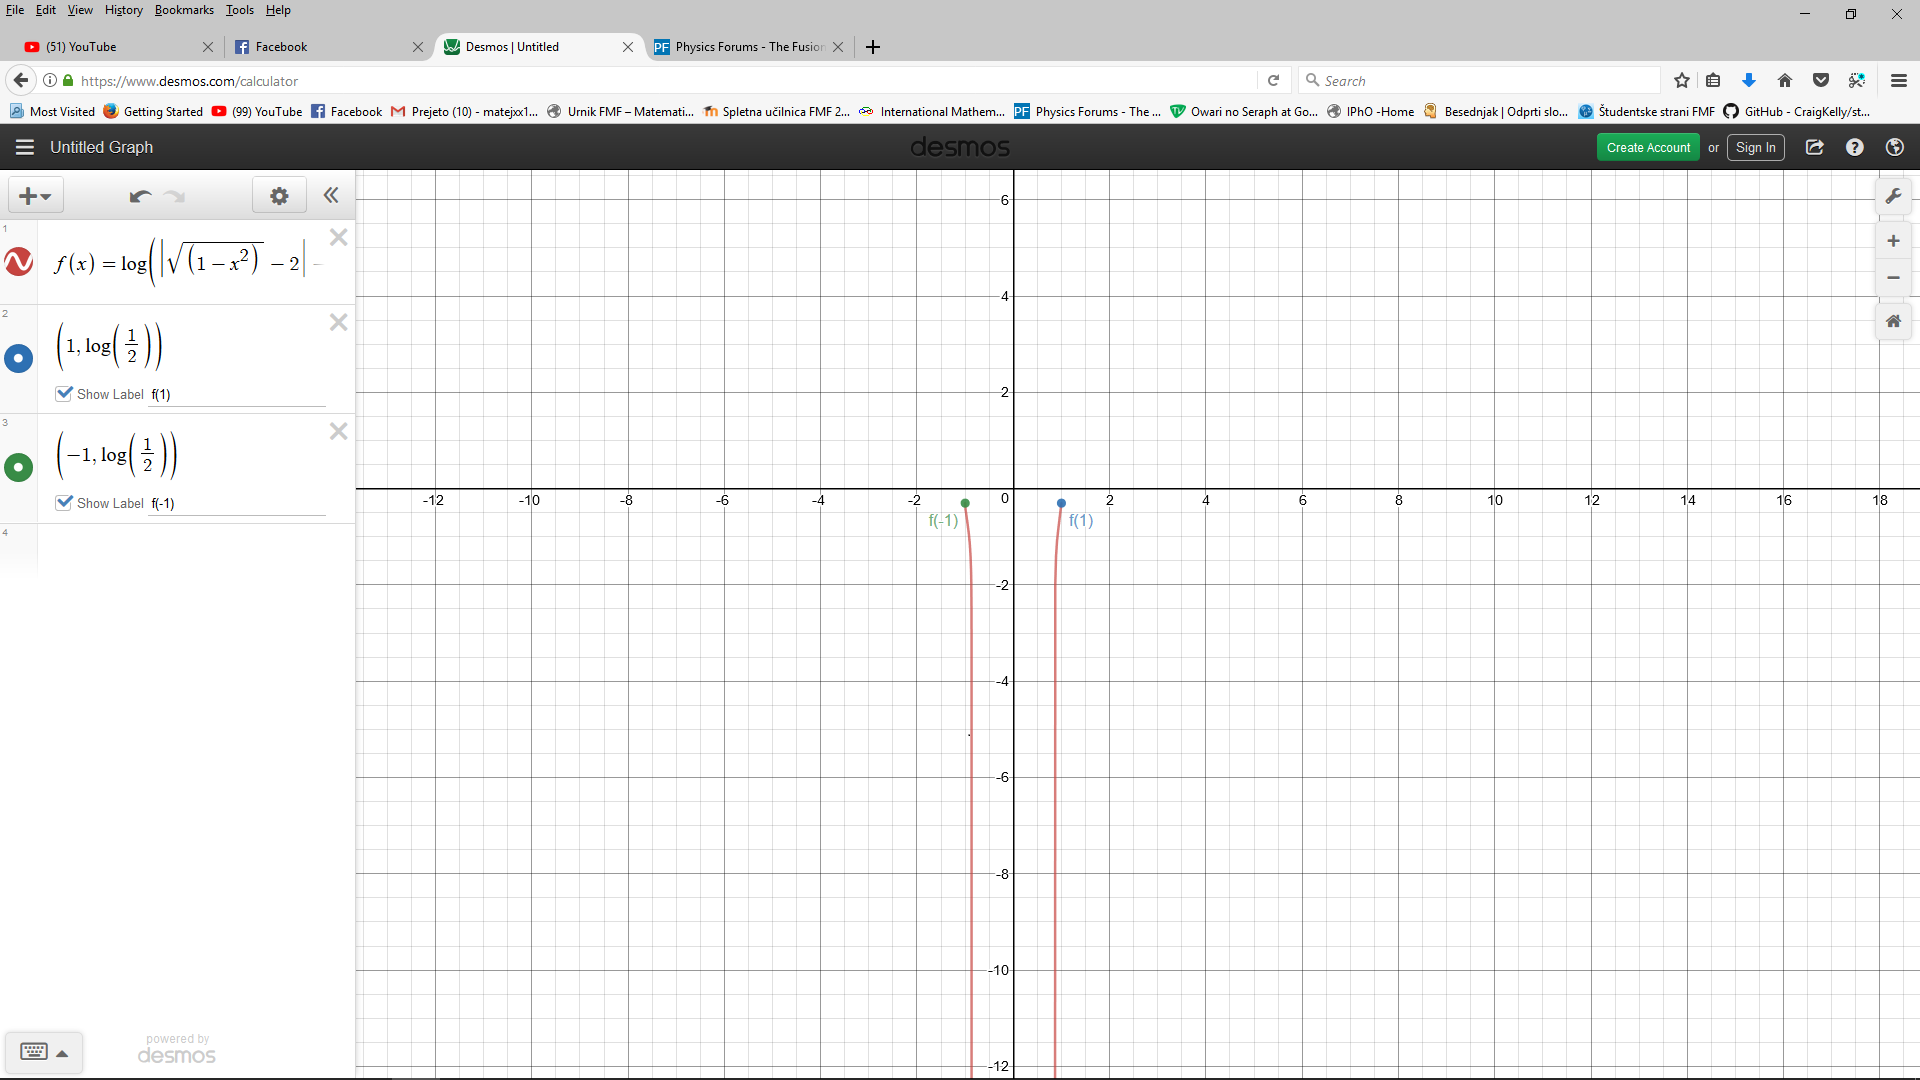
\includegraphics[width=\textwidth]{Funkcija.png}
\end{figure}
\end{itemize}

\end{document}